\documentclass{article}
\usepackage{v-equation}
\vgeometry
\usepackage{simpleopticss}
\def\foo#1#2{\number#1
    \ifnum#1<#2,
    \expandafter\foo
    \expandafter{\number\numexpr#1+1\expandafter}%
    \expandafter{\number#2\expandafter}%
    \fi}   

\begin{document}
\foo{5}{10}

\begin{center}
\makeatletter 
\define@key{cylindricalkeys}{angle}{\def\myangle{#1}} \define@key{cylindricalkeys}{radius}{\def\myradius{#1}} \define@key{cylindricalkeys}{z}{\def\myz{#1}} \tikzdeclarecoordinatesystem{cylindricall}%
{%
\setkeys{cylindricalkeys}{#1}%
  \pgfpointadd{\pgfpointxyz{0}{0}{\myz}}{\pgfpointpolarxy{\myangle}{\myradius}}
}

\def\pgfpointadd#1#2{%
 \pgf@process{#1}% 
 \pgf@xa=\pgf@x% 
 \pgf@ya=\pgf@y% 
 \pgf@process{#2}% 
 \advance\pgf@x by\pgf@xa% 
 \advance\pgf@y by\pgf@ya}
 
 
 
\makeatletter
\newcommand\xcoord[2][center]{{%
    \pgfpointxy{1}{1}%
    \@tempdima=\pgf@x
    \pgfpointanchor{#2}{#1}%
    \@tempdimb=\pgf@x
    \pgfmathparse{\@tempdimb/\@tempdima}%
    \num{\pgfmathresult}%
}}
\newcommand\ycoord[2][center]{{%
    \pgfpointxy{1}{1}%
    \@tempdima=\pgf@y
    \pgfpointanchor{#2}{#1}%
    \@tempdimb=\pgf@y
    \pgfmathparse{\@tempdimb/\@tempdima}%
    \num{\pgfmathresult}%
}}
\makeatother 
 
\begin{tikzpicture}[z=0.2pt]
  \draw [->] (0,0,0) -- (0,0,350);
  \foreach \num in {0,10,...,350}
    \fill (cylindricall cs:angle=\num,radius=1,z=\num) circle (1pt);
\end{tikzpicture}
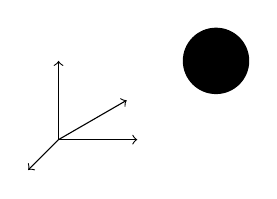
\begin{tikzpicture}[->]
  \draw (0,0) -- (xyz cs:x=1);
  \draw (0,0) -- (xyz cs:y=1);
  \draw (0,0) -- (xyz cs:z=1);
  \draw (0,0) -- (canvas polar cs:angle=30,radius=1cm);
  \coordinate (a) at (3, 4);
  \pgfpathcircle{\pgfpointadd{\pgfpoint{1cm}{0cm}}{\pgfpoint{1cm}{1cm}}}{12pt}
  \pgfusepath{fill}
  %\tzdot*(a)
  \newdimen\ex
\pgfextractx{\ex}{\pgfpointanchor{a}{center}}
%\tzdot*(\ex, \pgf@y)
%\tzdot*(\pgf@x, \pgf@y)
\end{tikzpicture}
\end{center}

\end{document}
